% CS 455, SP'22 Software development management plan
%
\documentclass[letterpaper,12pt,oneside,listof=totoc]{scrreprt}
\usepackage{listings}
\usepackage{graphicx}
%\usepackage{showframe} % visualize writing area and margins
\usepackage{underscore}
\usepackage{longtable}
\usepackage[bookmarks=true]{hyperref}
\hypersetup{
    bookmarks=false,                                 % show bookmarks bar
    pdftitle={Software Development Management Plan}, % title
%    pdfauthor={Yiannis Lazarides},                   % author
%    pdfsubject={TeX and LaTeX},                      % subject of the document
%    pdfkeywords={TeX, LaTeX, graphics, images},      % list of keywords
    colorlinks=true,                                 % false: boxed links; true: colored links
    linkcolor=blue,                                  % color of internal links
    citecolor=black,                                 % color of links to bibliography
    filecolor=black,                                 % color of file links
    urlcolor=purple,                                 % color of external links
    linktoc=page                                     % only page is linked
}%
\def\myversion{1.0 }

\date{\today}
\author{} % suppress warning, do not fill this in
\begin{document}

% we don't use \maketitle because we override the default title page here
\begin{titlepage}
\flushright
\rule{\textwidth}{5pt}\vskip1cm
\Huge{SOFTWARE DEVELOPMENT MANAGEMENT PLAN}\\
\vspace{1.3cm}
for\\
\vspace{1.3cm}
Data Storage System for Monitoring System\\
\vspace{1.3cm}
\LARGE{Release 1.0\\}
\vspace{1.3cm}
\LARGE{Version \myversion approved\\}
\vspace{1.3cm}
Prepared by Baxter Halder, Claire Hall, Kayla Jamar, Jennifer Olszyna\\
\vfill
\rule{\textwidth}{5pt}
\end{titlepage}

\tableofcontents % this will be automatically created from chapters, sections, and subsections
\listoffigures % this will be automatically created from the figure environment
\listoftables % this will be automatically created from the table environment

\chapter*{Revision History} % Update this table for each revision of the requirements
\begin{tabular}{| c | p{0.60\textwidth} | p{0.30\textwidth} |}
    \hline
    Date     & Description   & Revised by \\
    \hline
    02/16/22 & Initial draft & Data Store \\
    \hline
    02/21/22 & Revision of initial draft & Data Store \\
    \hline
    02/21/22 & Revision of draft & Data Store \\
    \hline
    03/2/22 & Final edits on draft & Data Store \\
    \hline
\end{tabular}

%----------------------------------------------------------------------------------------------------
\chapter{Introduction}

\section{Purpose} % what is the purpose of this document?
The purpose of this document is to give a detailed description of the requirements for the currently named “CS455 Monitoring System” software. This document will illustrate the purpose and complete declaration for the development of the data storage sub-system as well as explain the sub-system's: constraints, interface, and interactions with other external applications. This document is primarily intended to be proposed to a customer for their approval and act as a reference for developing the first version of the system for the development team.

\newpage
\section{Terminology}
\begin{longtable}{| p{0.40\textwidth} | p{0.50\textwidth} |} 
    \hline
   \textbf{ Term} & \textbf{Definition}\\
    \hline
    Admin/Administrator & System administrators are those with special privileges to managing and accessing the system. \\ 
    \hline
    Users & IT professionals who looks at the dashboard. \\
    \hline
    Agents & Software that continuously and autonomously collects specified information from client machines connected to the network for the monitoring system.\\ 
    \hline
    Engine/Monitoring Engine & Software on the network that will receives the data collected by the agents and continuously store it in the data storage. \\ 
    \hline
    Data Store/Data Storage & Database where the data collected by the agents is stored for the monitoring system to access. \\ 
    \hline
    Dashboard & a user interface that displays the collected data in the data storage to the admin.\\ 
    \hline
\caption{Definitions of Terms}
\end{longtable}

\newpage
\section{Acronyms} % define any uncommon acronyms you use in this document
\begin{longtable}{| p{0.25\textwidth} | p{0.65\textwidth} |} 
    \hline
   \textbf{ Acronym or Abbreviation} & \textbf{Definition}\\
    \hline
    KPI & Key Performance Indicators are quantifiable measure of performance over time for a specific objective that provides the admin insights into the network. \\
    \hline
    QA & Quality assurance is a system for evaluating performance. \\
    \hline
    GUI & Graphical User Interface\\
    \hline
    SRS & Software Requirements Specifications\\
    \hline
    UNA & University of North Alabama\\
    \hline
    CS455 & The computer science class at the University of North Alabama in which this project is being made\\
    \hline
\caption{Acronyms and Abbreviations}
\end{longtable}

\section{References \& Standards} 
% list (table?) of the applicable standards and relevant references
\begin{longtable}{ p{0.25\textwidth} p{0.60\textwidth} } 
   \textbf{ Standard} & \textbf{Reference }\\
    \hline
    TCP/IP &  \href{https://datatracker.ietf.org/doc/html/rfc1180}{RFC 1180}\\
    
    SQL and PL/SQL Coding Standards  & \href{http://www.dba-oracle.com/t_plsql_best_practices_standards.htm}{PL/SQL best practice Standards tips}\\
    
    Standard SQL Naming Conventions & \href{http://www.dba-oracle.com/standards_schema_object_names.htm}{Oracle naming standards tips}\\
    
    SEI CERT for C++ & \href{https://wiki.sei.cmu.edu/confluence/pages/viewpage.action?pageId=88046682}{SEI CERT Secure Coding Practices for C++}\\
\caption{References}
\end{longtable}

%----------------------------------------------------------------------------------------------------
\chapter{Project Overview} % brief description of the whole project
The CS455 Monitor System is a network monitor system that will monitor UNA's CS network in order to help administrators identify and address potential network problems as they occur. The system will automatically collect and store data, as well as provide warnings and error messages when certain events trigger the system. However, the system will rely on administrators to see the messages and act on them; the system is \textbf{not} automated to handle the events.  The monitor systems contains four sub-systems working in tandem; agents, monitoring engine, data store, and a dashboard.
This team's focus is the data storage unit of the system which will store the data collected by the agents.

\section{Software Overview} % description of the software component this team is building
The user will never directly interact with the database. The database acts solely as a place to store collected metrics and logs. The database will be scalable to accommodate up to hundreds of active servers and a dozen active dashboards. The database system will be hosted on UNA's CS server and host data for up to a year. The data storage will take data from the monitoring system and sort it into one of two two fundamental types of data, metrics or logs. 
Metrics are numerical values that describe some aspect of a system at a particular point in time. They are lightweight and capable of supporting near real-time scenarios. Logs contain different kinds of data organized into records with different sets of properties for each type.

\newpage
\section{Schedule} % planned schedule with activities including a nice chart
\begin{longtable}{| c | p{0.25\textwidth} | p{0.50\textwidth} |}
\hline
\textbf{Date} & \textbf{Item Due} & \textbf{Description} \\
\hline
02/11/22 & Client Consultation & Initial meeting with client to ask questions regarding client's initial request \\
\hline
02/16/22 & Initial draft & Initial rough draft of requirements document and software development management plan  \\
\hline
02/23/22 & Revision & Revised draft of requirements document and software development management plan \\
\hline
3/02/22 & Final draft & Final draft of requirements document and software development management plan \\
\hline
03/09/22 & Initial design review & Review initial design for software \\
\hline
03/16/22 & Implementation begins & Final design of software is completed and implementation begins\\
\hline
03/23/22 & Initial testing & Reviewing test plan and prototype \\
\hline
04/06/22 & Testing Phase 1 & Reviewing unit test results and prototype \\
\hline
04/13/22 & Testing Phase 2 & Reviewing unit test results and prototype after input from prior week \\
\hline
04/20/22 & Testing Phase 3 & Reviewing test results and prototype, then begin integration testing \\
\hline
04/27/22 & Integration and Acceptance Testing & Reviewing integration testing results and begin acceptance testing \\
\hline
05/03/22 & Software delivery & Deliver finished software and project deliverables \\
\hline
05/03/22 & Software Presentations & Team presentations (3:30 - 5:30) \\
\hline
\end{longtable}


\section{Budget} % type N/A for this section - describes the budget forecast for the product
N/A

\section{Project Deliverables} % list (table?) of the items that will be produced by the team for example, documents, manuals, databases, releases, etc.
The Data store team is responsible for producing a working SQL Database that is compliant with both the specifications set in this document and the SRS document.
The Data store team will all deliver all of the software and documentation associated with the data storage unit no later then May 3, 2022. A single copy of each of the deliverables listed below will be produced by the team.

\begin{longtable}{|p{.90\textwidth}|} 
    \hline
    \textbf{Name of Deliverable} \\
    \hline
    PDf of SRS document \\ 
    \hline
    PDf of SEI CERT Coding Standards documentation \\ 
    \hline
    Database system prototype to be used as data storage\\ 
    \hline
    Database system final version to be used as data storage\\ 
    \hline
    PDF of SDMP document \\ 
    \hline
    Software Design Document including a traceability matrix \\
    \hline
    Test plan document including a traceability matrix \\
    \hline
    Test results including a traceability matrix \\
    \hline
    User's manual for operating the software \\
    \hline 
    Software source code files \\
    \hline
    Copy of software version control repository \\
    \hline 
    Software executable \\
    \hline
    Team meeting minutes \\
    \hline
    Team communications summary document\\
    \hline 
    Copy of CM system data\\
    \hline
    PDF of presentation slides \\
    \hline 
\caption{Project Deliverables}
\end{longtable}



%----------------------------------------------------------------------------------------------------
\chapter{Management Approach} % org chart describing the overall management of teams working on project
\begin{figure}[h!]
\centering
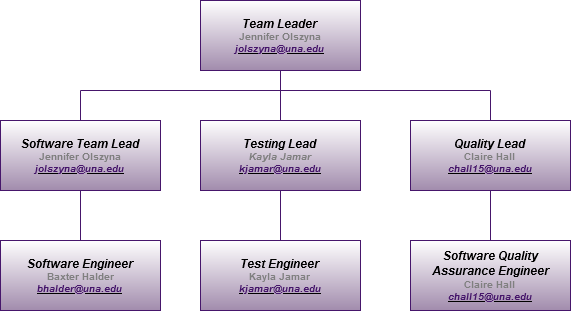
\includegraphics[scale=0.75]{Data Store Folder/org_chart.png}
\caption{Organization Chart Listing Project Roles}
\end{figure}

\section{Organization and Responsibilities} % each subsection describes a role and their responsibilities
% note - CM has a separate section
    \subsection{Software Team Lead} 
    A Software Engineering Team Leader is the member of the team who is responsible for their team’s execution, the quality they produce, the speed at which they produce. The Software Engineering Team Leader is also the member of the team who represents the team at the weekly stand-up progress report meetings.
    
    \subsection{Testing Lead} 
    The test leader plays an important role at an outset of the project.Test leaders collaborate with other stakeholders, devise the test objectives, organizational test policies, test strategies and test plans. They decide when test automation is appropriate and they put effort and plan to select the tools and ensure training the testing team. The team leader is also responsible of making sure the test environment is set up and verified before test execution.
    
    \subsection{Quality Lead} A Quality Lead is responsible for the management and organization of quality testing. They ensure that a project will have a successful promotion by providing quality software and testing the product to ensure that it follows according to the guidelines. They are also involved in finding a solution to any conflicts between teams, and they give motivational advice for the team. 
    
    \subsection{Software Engineer} 
    Software engineers design and create computer systems and applications to solve real-world problems. Software Engineer know how to use the right programming languages, platforms, and architectures to develop everything from computer games to network control systems. In addition to building their own systems, software engineers also test, improve, and maintain software built by other engineers. 
    
    \subsection{Test Engineer} 
    Software test engineer has the role of coordinating the process for analyzing software programs. This process will involve creating and implementing testing methods, recording the test results, and providing recommendations to improve software programs based on the results. Test engineers should be tasked with interfacing with end users to ascertain areas of improvement, such as cost reduction solutions and automation solutions.
    
    \subsection{Software Quality Assurance Engineer} 
    A software quality assurance engineer monitors every phase of the development process to ensure that the design and software adhere to company standards.
    A software quality assurance engineer perform the following tasks with some regularity:document test cases and risk analysis, record test progress and results, lead team on overall testing processes(both manual and automated ), identify any potential problems that users might encounter.
        
\newpage
\section{Software Risk Management} % list risks to the project and describe how the project will identify, track, and mitigate risks
The risks below are broken up into the three subcategories of process risks, programmatic risks, and technical risks. 

\subsection{Process Risk Management} 
Process risks are problems arising from improper process implementation. 
\begin{longtable}{| p{0.30\textwidth} | p{0.30\textwidth} | p{0.30\textwidth} |} 
    \hline
    \textbf{Risk} & \textbf{Description} & \textbf{Mitigation Strategy} \\
    \hline
    Semantic Risks & Data is mis-stored in wrong field & data migration testing\\
    \hline
    Extended Downtime Risk & Data transfer from engine take longer then allotted time & Alert engine, and attempt to retry transfer\\
    \hline
\caption{Software Process Risk Management}
\end{longtable}

\subsection{Programmatic Risk Management} 
Programmatic risks include things like schedule, resources, and mismanagement. 
\begin{longtable}{| p{0.30\textwidth} | p{0.30\textwidth} | p{0.30\textwidth} |} 
    \hline
    \textbf{Risk} & \textbf{Description} & \textbf{Mitigation Strategy} \\
    \hline
    Inadequate Knowledge & Member(s) are unaware or familiar with SQL & Make sure all members are trained in SQL and \\
    \hline
\caption{Software Programmatic Risk Management}
\end{longtable}

\newpage
\subsection{Technical Risk Management} 
Technical risks are threats to the quality, security, and performance of the software. 
\begin{longtable}{| p{0.30\textwidth} | p{0.30\textwidth} | p{0.30\textwidth} |} 
    \hline
    \textbf{Risk} & \textbf{Description} & \textbf{Mitigation Strategy} \\
    \hline
        Data Corruption & Unintended changes or errors in data that occur during transfers or storage of the data. & Utilize the log files of SQL Server to restore the database. \\
    \hline
    Data Loss & Incomplete data transfer or un-explainable loss of data & Data migration, reconciliation testing in instance of system errors or detected loss\\
    \hline 
    Data Leakage & Data loss of sensitive information & implement a Password Security Policy\\
    \hline
    Inadequate Space & Data amount exceeds allotted database storage & Give alert to Dashboard when at 95 percent storage capacity\\
    \hline 
    Interference risk & Multiple users attempting to access data base simultaneously & data store will limit concurrent user assesses\\
    \hline
\caption{Software Technical Risk Management}
\end{longtable}


\section{Customer Communications} % describe how the project will communicate with stakeholders
A weekly stand up meeting with all members of project where software team leads of each division will summarize weekly activities and plans for the upcoming week. Meeting notes will be recorded by the team and stored in the project repository.
    
\newpage
\section{Team Training} % list and describe any required training for team members detail how required training will be documented and reported. For example, secure coding training or tools training
There is no explicitly defined team training plan for this project. The main training sources for this project are the UNA program courses, which include training in the following areas: Methods of software development, software architecture, analysis of software artifacts, management of software development, models in software development, and optionally Database systems. As database systems was not a required course, those on the team not familiar with the domain will need to familiarize himself or herself with the basics of Database Management Systems

\begin{longtable}{| p{0.20\textwidth} | p{0.40\textwidth} | p{0.13\textwidth} | p{0.12\textwidth} |} 
    \hline
    \textbf{Training Type} & \textbf{Description of Training} & \textbf{Member} & \textbf{Date}\\ 
    \hline
    Basic SQL Training & Basics of SQL scripts & Entire Team & \\
    \hline 
    Basic Database Training & Theories and applications of database system course at UNA & Entire Team & 12/07/21\\
    \hline 
    Secure Coding Training & Basics of secure coding standards set by SEI CERT & Entire Team & 2/16/22\\
    \hline 
\caption{Training}
\end{longtable}



%----------------------------------------------------------------------------------------------------
\chapter{Technical Approach} % this section describes the team's software engineering process
% each section describes how the named item will be managed, tracked, documented, and reported

\section{Development Process}
% process used by the team to develop the software
% including a coding standard and a secure coding standard
% may also (should include) peer code reviews
The team plans to use the standard data language Structured Query Language, specifically MySQL. MySQL is an open-source relational database management system. The relational database will organizes data passed to it from the engine into one or more data tables in which data types are related to one another to structure the data. The standard SQl names and coding conventions will be used. Code will be broken into components, and each member will take responsibility for a component. 
Peer review will be periodically done by other members of the team.
Peer reviews purpose is to remove defects as early as possible in the development process. The process includes removing defects in the original documents such as the requirement and design documents, test plans and procedures.
The peer should be someone that is a technical expertise and equal standing, while the review should involve the careful judgement. The process begins with a determined scope of review.Next, a determine rigor level leading a plan to review in detail. finally, we ensure observations are resolved.
The team makes an effort of considering all requirements within reviews.Reviews are sent to the technical expertise for missed expectations once discussed by entire team. Those mistakes will be corrected every week leading to useful product.

\section{Development Tools}
% software tools, for example IDE's, compilers, test tools, static analysis, version control, etc.
The standard Windows and Linux OS terminal, build in compiler and online IDE environment's compiler will be used as development tools.

\section{COTS \& FOSS Tools}
% commercial-off-the-shelf (COTS) software used and open source software used in the product
% note - these create risks
% (FOSS)software that is both FREE  and OPEN-SOURCE SOFTWARE where anyone is freely licensed to use, copy, study, and change the software in any way,
As the data storage unit will be created using the MySQL relational database management software, the main environment will be the terminal. The team will utilize the MariaDB monitor that is already available on the CS network.
MariaDB is a open-source GNU General Public License community-developed, commercially supported fork of the MySQL relational database management system, 

\section{Software Reuse}
% describes any software that was previously produced by the team that is being reused in the product
% note - these create risks
N/A

\section{Testing Process}
% describe the plan for testing the software meets requirements
% include how tests and test results are documented, tracked, and reported
The team plans to use standard SQL testing to check that the database works as it should.
blank will be done to ensure compliance with the SEI CERT style guide.
Communication and accessibility tests will be conducted first. The team will test to see if the data store can communicate with the engine and the dashboard over the network. They will also test to see if the user can interact with text forms of the data from the dashboard. Once communication and accessibility tests have been passed, testing will move forward to the next step. Information retrieval and view-ability tests will be conducted next. The team will then test to see if system administrators can retrieve information regarding CPU usage, memory usage, disk usage, and network usage from the data store. Once information retrieval and view-ability tests have been passed, scale-ability and longevity tests will be conducted. The team will test to see if the system will be able to scale up to at least fifty servers. They will also test to see id data will be able to be stored for at least a year. Once scale-ability and longevity tests have been passed, data transfer tests and sanity checks will occur. The team will test to ensure that only valid data, not invalid data, makes it through the management engine to the data store. Once data transfer tests and sanity checks have been passed, dependability and security checks will be conducted. The team will test the fault tolerance of the system. They will also test to see if information can be be saved and sent again if the server goes down. For more detailed information, please refer to the Data Store Test Plan. 


%----------------------------------------------------------------------------------------------------
\chapter{Configuration Management}
% describe how configuration management will work in the project
%everything that gets generated is a configuration item / record and document Configuration item

\section{CM Responsibilities}
% detail who is responsible for each aspect of CM
% what are responsibilities of that person, make sure people do what their supposed to do
The configuration management will fall to the software assurance engineer. The responsibilities of a configure manager consists of plan and execute CM throughout the project lifestyle, including development, migration, deployment and security. They also identify, organize, and control software and hardware configuration changes.

\section{CM Resources}
% list the tools used for CM, for example software used to track and report CIs
Tools for CI would include, Overleaf LaTex for the documentation and the messaging platform Discord for communication outside meetings.

\section{Change Control Procedures}
% describe the process for managing changes to the software product
% can't commit changes until unit tests, or verified by people, etc.
% version control software 
Notes are taken at weekly meetings detailing the minutes and topics discussed.

%----------------------------------------------------------------------------------------------------
\chapter{Verification \& Validation}
% describe how the team will know the product is complete (detail acceptance criteria)
% verification - did we build the product right?
% validation - did we build the right product? 

\section{V\&V Procedures}
% describes the verification and validation procedures
The verification process will be a series of tests specified in the project SRS that show the product works. Then the validation process will be a series of tests specified in the SRS that show the product build is what was intended for the greater project.
% translate graph into paragraph

\section{Independent V\&V}
% type N/A for this section - used when an independent group performs V&V in addition to the team's V&V
N/A

\end{document}




